

%% EINLEITUNG %% 
\chapter{Fundamentals}
This section explains basics needed to understand the rest of the work. Since the Flutter framework and the Dart programming language with which this application is to be developed are not topics that are dealt with in a computer science degree, they will also be discussed.

\section{Flutter and Dart}
The framework used to develop the disease-detection application will be Flutter, which is an open-source-UI-Kit developed by Google. Flutter uses the open-source programming language Dart, which at first was designed for building Google Chrome browser-applications and later on benefited greatly from various improvements since it was released back in 2011. The programming language consequently evolved from having a lot in common with JavaScript to sharing many features with C\# and Java. The Flutter and Dart ecosystem, which is brimming with open-source packages created by other developers from around the world, is one of the framework's best features. It enables programmers to create visually stunning applications in the shortest amount of time, by including packages from developers all over the world. Also, Dart is a client-optimized gneral-purpose programming language that supports cross-platform development. This implies that this application will be created with a single code base yet will run on both Android- and iOS-smartphones. Furthermore, the program may be launched as a web application and utilized on embedded devices. However, as part of the bachelor thesis, the development and testing process will be entirely focused on Android development. Dart is also a statically-typed language, which means that the type of each variable must be explicitly declared, making it easier to catch bugs and other issues early on in the development process. With null safety, Dart ensures that variables cannot be assigned a null value unless they are explicitly declared as nullable. This means that if a variable is expected to have a non-null value, it must be initialized with a non-null value, and any attempts to assign a null value to it will result in a compile-time error. This helps prevent null reference errors and makes it easier to write code that is safe and predictable. [QUELLE:DART/OVERVIEW]

\subsection{Flutter: Everything is a Widget}
When researching how Flutter functions, it's common to come across the phrase "In Flutter, everything is a widget." The difference between Flutter's widgets and those in other Frameworks' components is that Flutter's widgets can specify how the application's user interface should appear. Eric Windmill was able to divide the widgets into various groups in his book Flutter in Action [flutter in action, s 58]:

\begin{itemize}
	\item \textbf{Layout:} 
	Widgets of this category are able to store children-widgets, an example for such a widget would be a row, column or even a stack.  
	\item \textbf{Structures:} 
	As their name implies, structures aid in organizing the application.
	For instance, MenuDrawer produces a sidedrawer for the application, toasts display a message to the user, and buttons can respond to various click patterns. 
	\item \textbf{Styles:} 
	The developer can style widgets in almost any way using Flutter. With a tool like ButtonStyle, a button's background and foreground colors as well as its shape can all be changed.
	\item \textbf{Animations:} 
	Flutter enables its users to breathe life into their applications with a rich palette of animation options. For instance, Flutter developers can use well-known animation features like curves, which are also used in CSS. 
	\item \textbf{Positioning and Alignment:} 
	Widgets such as Padding and Center allow it to position its child widget. There are also additional widgets, such as Positioned and Alignment, that allow the developer to position elements in a Stack.
\end{itemize}
\noindent 
The categorization created by Eric Windmill provides a decent overview of the possibilities in Flutter. There are undoubtedly a lot more widgets and a lot more usage categories that might be defined. Widgets can be composed, which means nested inside of one another [Flutter in action, s61], so rather than simply returning the widget it describes, a widget's build method really returns a tree of widgets. The DOM in any web browser is comparable to this widget tree. A sample widget returned by a build method is shown in Listing 2.1. Figure 2.1 illustrates the generated widget tree in detail.
\begin{lstlisting}[caption=Flutter Scaffold Example]
	Widget build(BuildContext context) {
		return Scaffold(
			appBar: AppBar(
				title: const Text('Example of the build method'),
			),
			body: const Center(
			child: Text('Hello Reader'),
			),
		);
	}
\end{lstlisting}
\begin{figure}[H]
	\centering
	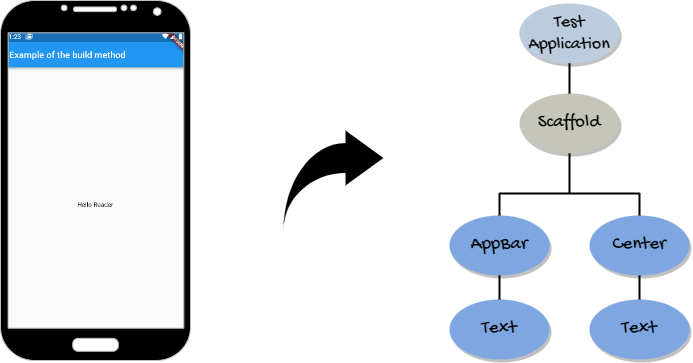
\includegraphics[scale=0.45]{widget_tree.png}
	\caption[Widget Tree of Listing 2.1]{Widget Tree of Listing 2.1}
\end{figure}
\subsection{Flutter: Architectural Layers}
A well-designed application architecture helps improve the systems performance, maintainability, scalability but also makes it more modular. [Buch: Software arhcitecture seite 28] Many different application architectural patterns can be used, including layered architecture of which Flutter makes use.  In the context of software development, layered architecture is a common design pattern in which the application is divided into different layers, each layer plays a specific role in the overall functionality of the application. [Flutter.dev architectural layers] The Flutter architecture includes a number of key components, including the Flutter engine, the Dart platform and the Flutter framework. The Flutter engine is responsible for rendering widgets and managing their interactions with the underlying platform, such as the operating system and device hardware. The Dart platform provides the runtime environment for the Flutter app, including the Dart virtual mavhine (VM) and the core libraries. Application architecture refers to how the various components of a mobile or web application are organized and how they interact with each other. No layer has privileged access to the layers below, and every part of the framework layer is designed to be optional and interchangeable. Figure x.x shows the basic structure of a Flutter application. 
\begin{figure}[H]
	\centering
	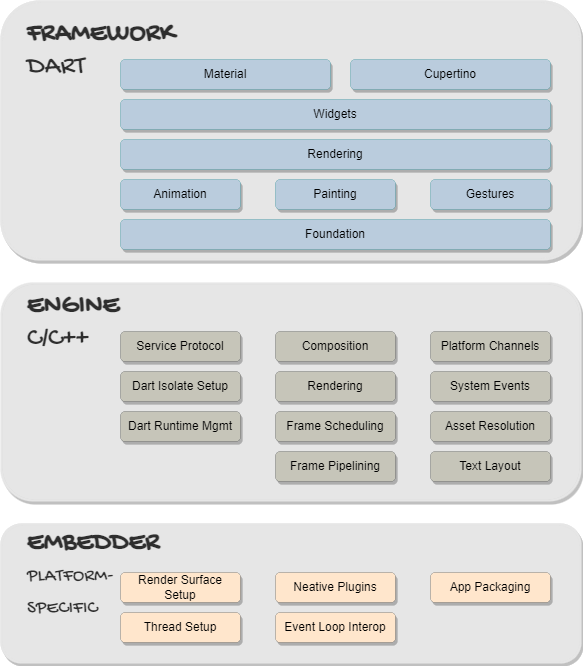
\includegraphics[scale=0.45]{layered_architecture.png}
	\caption[Layered Architecture in Flutter]{Layered Architecture in Flutter[based on Flutter page and TakingFluttertotheWeb page 50/]}
\end{figure}


\subsection{Programming Paradigm}
The programming paradigm of the Dart programming language is object-oriented programming (OOP). This means that it uses objects, classes, and inheritance to organize and structure code. Dart also incorporates some functional programming concepts, such as immutable data and first-class functions, which allow for more concise and elegant code. Additionally, Dart supports asynchronous programming, which enables developers to write code that can run concurrently and handle multiple tasks at the same time. Overall, Dart's combination of OOP and functional programming paradigms makes it a versatile and powerful language for building modern web and mobile applications. The SOLID principles are a set of guidelines for designing object-oriented software. They were introduced by Robert C. Martin in his book "Agile Software Development, Principles, Patterns, and Practices" as a way to improve the maintainability, extensibility, and flexibility of object-oriented code and to develop software that is prone to fewer bugs and has cleaner source code. [https://www.freecodecamp.org/news/solid-principles-explained-in-plain-english/] These principles should be taken into account when developing the application.
\begin{itemize}
	\item \textbf{Single Responsibility Principle (SRP):}
	The single responsibility principle instructs the developer to develop classes and software components in such a way that they take on a maximum of one responsibility. In other words, a class should focus on a single task or piece of functionality, and should not be responsible for multiple unrelated things. This helps to reduce complexity and improve the maintainability, testability, and extensibility of a software system. Another positive side-effect of following this principle is that the written code is easier to understand and error-testing can be done more efficiently.
	
	\item \textbf{Open/Closed Principle (OCP):}
	According to the open-closed principle, software classes should be open for extension but closed for modification, which means a class should be designed in such a way that it can be easily extended or customized without changing its existing code. This allows developers to add new features or behaviors to a class without breaking its existing functionality. This suggests that these classes or software components ought to be developed in a way that allows other system entities to use their essential features without requiring access to the original entity's source code. 
	
	\item \textbf{Liskov Substitution Principle (LSP):}
	The Liskov Substitution Principle (LSP) asserts, in essence, that whenever a function uses a pointer or reference to a base object, it must also use a pointer or reference to any of its derived objects. [Software architecture with c++] One can also say, that it is an extension of the OCP. A subclass should be able to be used wherever its superclass is expected, without breaking the functionality of the program. [stickify, solid design liskov] The Liskov Substitution Principle helps to improve the flexibility and reusability of a software system.
	
	\item \textbf{Interface Segregation Principle (ISP):}
	The Interface Segregation Principle ensures that a clients of a class should not implement an interface that contains methods that are not relevant to its functionality. This helps to avoid creating large and complex interfaces that are difficult to implement and maintain. The Interface Segregation Principle promotes the creation of small, focused, and easy-to-use interfaces. 
	
	\item \textbf{Dependency Inversion Principle (DIP):}
	The key essence of the DIP is that a class should not depend on the specific implementation details of another class. Instead, it should depend on an abstract interface or a set of contracts that define how the two classes should interact.
\end{itemize}

\section{Application Programming Interfaces}
The aim of this work is the conception and implementation of the described system. In order to achieve this goal, the application must access a database that is filled with suitable data. The information from an existing application programming interface (API) is used here, since there are no medically trained project participants who could contribute their specialized expertise to the database. The final data structure of the database is also influenced by the selection of the API. For this purpose, the two most suitable APIs are considered and their suitability for the project is determined
\subsection{NHS Health A to Z API}
The NHS, or National Health Service, is the publicly funded healthcare system of the United Kingdom. It was established in 1948 and provides a wide range of medical services to the population of the UK, including general practitioners (GPs), hospitals, and community health services. The NHS websites provides many different APIs, free for use [NHS website]. The NHS Health A to Z API is the first API that will be considered to generate data for the database.
The API offers medical information about various diseases, their symptoms, and available treatments. A user account that is provided with a subscription key must be created in order to receive data from this API. The next step is to make an HTTP call to https://api.nhs.uk/conditions. An example of a possible request in the programming language Python looks like this:
\begin{lstlisting}[language=Python, caption={Example Python Request for the Health A to Z API}]
urlDiseases = "https://api.nhs.uk/conditions/acne"
header = {
	"subscription-key" : "YOUR_SUBSCRIPTION_KEY"
}
responseDiseases = requests.request("GET", urlDiseases, headers=header)
responseData = responseDiseases.json()
\end{lstlisting}
If the request was successfull and the response contains the data in JSON format. Listing 2.3 shows a sample abbreviated response from the API.
\begin{lstlisting}[caption={Example Response for the Health A to Z API}]
{
	"@context":"http://schema.org",
	"@type":"MedicalWebPage",
	"name":"Acne",
	"copyrightHolder":{...},
	"license":"https://developer.api.nhs.uk/terms",
	"author":{...},
	"about":{...},
	"description":"...",
	"url":"https://api.nhs.uk/conditions/acne/",
	"genre":[...],
	"keywords":[...],
	"lastReviewed":[...],
	"breadcrumb":{...},
	"dateModified":"2022-05-30T14:30:18+00:00",
	"hasPart":[...],
	"relatedLink":[...],
	"contentSubTypes":[...],
	"mainEntityOfPage":[...],
	"alternativeHeadline":"Overview"
}
\end{lstlisting}
An entire text document with the server's response to the request made in listing 2.2 can be viewed by scanning the QR code shown in the appendix x.x. A positive aspect of this API is that all data is described in great detail and a large amount of knowledge can be obtained in a single query. However, it must also be mentioned that the extent of the server response just mentioned entails the difficulty of storing the data accordingly in a separate database. For example, symptoms are supplied for a disease, but only in string format as a complete sentence. This means that a symptom is described in different ways in several diseases. In order to automatically scrape this data, one would have to recognize all variations in the description of a symptom. With the amount of data that the Health A to Z API brings with it, this is almost impossible. Another limitation is that a maximum of 6 requests can be made to the interface per minute, which proves to be a serious problem in terms of runtime.

\subsection{ApiMedic Symptom Checker API}
The ApiMedic API is the second interface to be considered. ApiMedic is powered by priaid, a company that focuses on bringing together medicine, IT and business administration. Thanks to their highly specialized team composition, they offer expertise in all of the areas mentioned. The API can be addressed in two different ways:
\begin{itemize}
	\item \textbf{Sandbox API Account:}
	It is possible to get an unlimited amount of data via the sandbox account. However, the data supplied is only dummy data.
	\item \textbf{Live Basic API Account:}
	The live account allows to get the actual medical data of the API. However, there is a limitation with regard to the possible calls: ApiMedic only allows 100 calls per month to be made without charging money, further requests cost money.
\end{itemize}
Although the data that can be received from this API is not as detailed as that of the NHS API, using the data to create a data structure is simpler. It is possible to acquire diseases, bodily components, and symptoms as well as proposed symptoms and symptoms based on each body part. The following code example shows an request, made with the live account, to retrieve all diseases followed by the response of the API.
\begin{lstlisting}[language=Python, caption={Example Python Request for the ApiMedic API (all issues)}]
stringURLIssues = "https://healthservice.priaid.ch/issues?token=YOUR_TOKEN"
responseIssues = requests.request("GET", stringURLIssues)
dataIssues = responseIssues.json()
\end{lstlisting}

\begin{lstlisting}[language=Python, caption={Response for the ApiMedic API (all issues)}]
[
	{
		"ID": 130,
		"Name": "Abdominal hernia"	
	},
	{
		"ID": 170,
		"Name": "Abortion"	
	},
	{
		"ID": 456,
		"Name": "Abscess of the tonsils"	
	},
...
\end{lstlisting}
It is now possible to execute an API request that returns detailed information about each disease, using the provided IDs. Listing 2.7 shows a sample shortened response from the ApiMedic API.
\begin{lstlisting}[language=Python, caption={Example Python Request for the ApiMedic API (single issue)}]
	stringURLIssue = "https://healthservice.priaid.ch/issues/105/info?token=YOUR_TOKEN"
	responseIssue = requests.request("GET", stringURLIssue)
	dataIssue = responseIssue.json()
\end{lstlisting}

\begin{lstlisting}[language=Python, caption={Response for the ApiMedic API (single issue)}]
{
	"Description": "Measles is caused by a virus a...",
	"DescriptionShort": "Measles, also known as morbilli, ...",
	"MedicalCondition": "The infection begins with flu-like symptoms ( ...",
	"Name": "Measles",
	"PossibleSymptoms": "Burning eyes,Burning in the throat,Cough,...",
	"ProfName": "Morbilli",
	"Synonyms": "Red measles",
	"TreatmentDescription": "To prevent measles, an effort to vaccinate ..."
}
\end{lstlisting}
\noindent 
The value of the "PossibleSymptoms"-key returns an enumaration of all the symptoms of the disease. These symptoms are listed using the values of the "Name"-key for the respective symptom when querying all symptoms. This makes it easier to scrape the data accordingly and store it in a database.

\subsection{Conclusion}
The question that now arises is which of the two interfaces to choose. Both APIs have advantages and disadvantages. While the NHS API provides very detailed results, it makes it difficult to use the data for the purposes intended in this work. NHS also provides data on the causes that various symptoms and conditions can have, which can be an important factor in making a diagnosis in the form of disease detection. ApiMedic delivers the data in an optimal format to use, but far less detailed than NHS. One option that is available is, to use the symptom data provided by ApiMedic as scrape material for the symptom list in the NHS. However, after an attempt to do so, only a very small amount of symptom has been recognized. This is because the same symptom is named differently in both APIs. Generating more appropriate scrape material would require full inspection of all NHS API data, to ensure getting a decent amount of data. This is not possible within the scope of this work, but should be considered for future optimizations of the system.  In the context of the bachelor thesis, the use of the ApiMedic API is preferred from the point of view of a clean database structure.

\section{NoSQL Databases}

\subsection{Introduction to NoSQL Databases}
The generic term NoSQL describes database systems that, unlike SQL databases, are not subject to the relational database model. The abbreviation NoSQL stands for "Not only SQL". The reasons why NoSQL databases have gained interest in recent years can be explained on the basis of two aspects: In contrast to relational databases, which present their data storage in table format, NoSQL databases benefit from different database models: document-oriented, key Value, graph and column databases.[Image] This wide range of different data models gives developers the benefit of being able to choose the model that best suits their application design. The resulting result is a minimization of the code to be developed for an application. In addition, NoSQL databases allow administrators to scale their data both on one machine and on hardware clusters, so data volumes can be expanded without an expensive investment in new servers.
\begin{figure}[H]
	\centering
	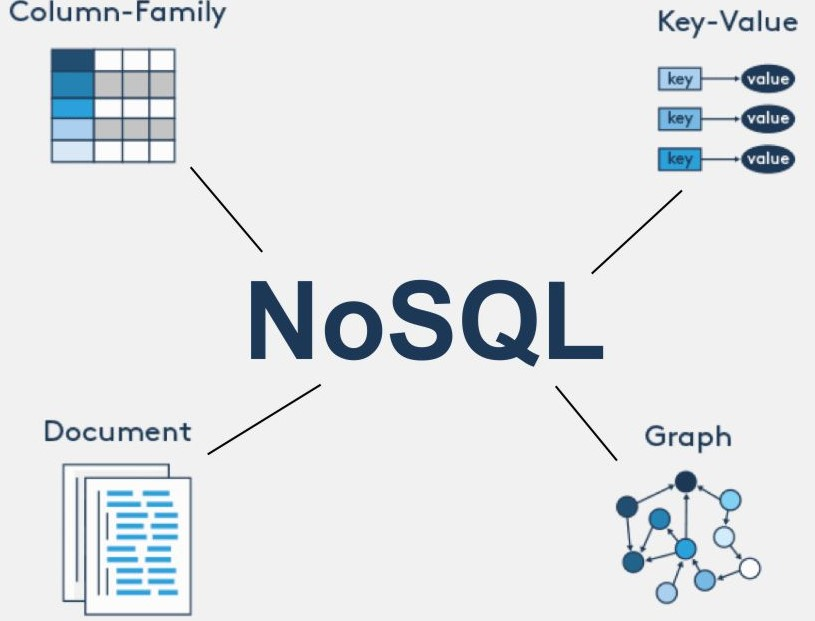
\includegraphics[scale=0.25]{nosql.jpg}
	\caption[NoSQL Data Models]{NoSQL Data Models}
\end{figure}

NoSQL databases support the use of CRUD operations.
\begin{itemize}
	\item \textbf{C:} create data
	\item \textbf{R:} read data
	\item \textbf{U:} update data
	\item \textbf{D:} delete data
\end{itemize}
The performance of some NoSQL databases even surpasses that of relational databases, especially with create and read operations. [Performance evaluation for CRUD] A detailed  performance comparison can be found in Appendix [Performance evaluation for CRUD].
\subsection{Firestore}
Cloud Firestore, more often called Google Firestore, is a cloud-hosted NoSQL database option which enables developers to store and synchronize their data in realtime, meaning that data which just got added to the database and changes made on already existing data are instantly shown to the application users. It is a part of Googles Backend-as-a-Service (BaaS) Firebase. BaaS is a concept where developers can use a platform to run their applications without managing servers and other infrastructure components. BaaS platforms offer a range of services required for applications to run, such as databases, authentication, storage and APIs. [okta.com] To use BaaS, developers must first create an account with a BaaS platform and register their application on it. The platform then provides a set of APIs and SDKs that developers can use to access the services and integrate them into their application. Most BaaS platforms offer a web-based console that developers can use to manage their applications and configure the services, so does Firebase. Since Firestore is published by Google, it comes with peak reliablitly and great performance. Something worth to mention is, that Firestore can be used with far more programming languages than Dart and is also compatible with REST and RPC APIs. [firestorewebsite] Cloud Firestore caches data that your app is actively using, so the app can write, read, listen to, and query data even if the device is offline. When the device comes back online, Cloud Firestore synchronizes any local changes back to its servers. To keep your data safe, firestore offers the opportunity to create security rules based on an individuals needs, this includes Identy and Access Management (IAM). Using firestore combined with the flutter framework one can retrieve data via the cloud\_firestore-plugin. It enables the developer to make use of the cloud firestore API. The named package also allows the developer to make use of the authentication functionality provided by the BaaS, which makes it possible for a user to register and login in an application. When trying to get data with a flutter application of a firestore database, one can simply set the GetOptions-Parameter. With defining the parameter source, one can first check, if the required data is already in the devices' cache. An example is shown in Figure 3.8.

\begin{lstlisting}[language=Python, caption={Dart - Firestore-Query}]
	
Future<DocumentSnapshot> checkCacheBeforeServer() async {
	try {
		DocumentSnapshot snapshot = await this.get(GetOptions(source: Source.cache));
		if (snapshot == null) return this.get(GetOptions(source: Source.server));
		return snapshot;
	} catch e {
		print(e);
		return this.get(GetOptions(source: Source.server));
	}
}
	
\end{lstlisting}
\noindent

\subsection{Document Databases}
There are several different NoSQL databases, which all rely on different data models. Firestore makes use of the document-based data format. This means, that data stored in the database is accessible via collections, which are filled with documents. For better understanding one can imagine a collection in Firestore as a table in relational Databases and a Document in Firestore equals a row in the relational schema. An example of that is shown in the figure x.x. Documents in Firestore store their data in a key-value-format which makes it possible for a developer to store different sort of documents in each collection. A quick view at an example makes this easier to understand: A developer wants to develop a restaurent-review application. For that he creates a collection named “restaurants” in firestore. Two of the three restaurants he now wants to add to the collection got a slogan with their brand which he wants to add to the documents, the other restaurant doesn’t have one. In a relational database he still would have to fill the “slogan” column with at least NULL-data or an empty String (or whatever datatype the column has). Firestore, or document-based databases in general, allow it, to just not add the slogan attribute to the third restaurant, which helps to only store relevant data to the database. One thing to keep in mind is, that even if the third restaurant one day gets a slogan, the developer has the possibility to add that field to the document later on. Cloud Firestore also allows it to store subcollections or complex nested objects to documents. Firestore has no option to store foreign keys in a document. The solution to create a foreign key-like mechanism is covered in the Database chapter. 